\chapter{Programming the Signature and Validation of Several DNSSEC Resource Records}
\label{chap:prog-chapter}

\section{Main Functionality}

There are several arguments that can be passed to the program: 
\begin{enumerate}
  \item The first argument is the name of the file that contains the private key that will be used for signing.
  \item The second argument is the name of the file that contains the public key that will be used for verifying the signature.
  \item The third argument is the name of the file that contains the hexadecimal representation of the data to be signed.
  \item The final argument is the name of the file that will contain the signature from the server in Base64 format.
\end{enumerate}

This list of inputs is seen below in the code and comments in \cref{fig:input}. This is an early catch to prevent any other 
errors from occurring down the line, while also ensuring a clean input is received.

\begin{figure}[htbp]
  \centering
  \fbox{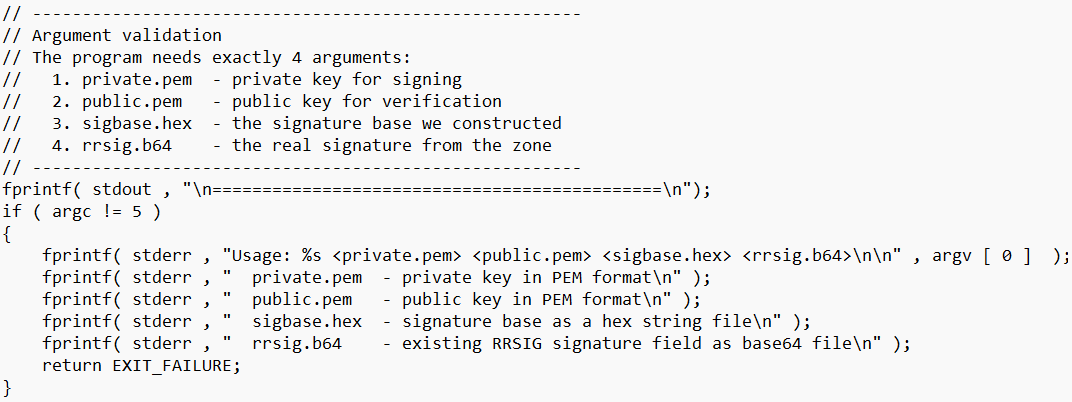
\includegraphics[width=0.8\textwidth]{code/input.png}}
  \caption{A snippet of code at the top of the main function, validating the input and providing a helpful message to make sure the user inputs the correct elements in the correct order.}
  \label{fig:input}
\end{figure}

\FloatBarrier

Using these arguments, the data is read into buffers in the program, and the base64 signature is read in, converted to binary, 
and stored in a buffer as well. Firstly, a signature is generated using OpenSSL's EVP\_DigestSign family of functions, seen 
below in \hyperref[sec:signing]{Signing the Data} section, \cref{fig:signing-code}. The signature base, or hexadecimal notation 
of the data to be hashed, is passed in here and stored as the generated signature. This signature is then passed to another family 
of OpenSSL functions, EVP\_DigestVerify, seen in \hyperref[sec:verify-code]{Verifying the Signature}, \cref{fig:gen-verification-code}
which uses the public key to cryptographically verify the signature. The same happens with the existing signature that was queried 
from the server, seen in \cref{fig:existing-verification-code}. After these verifications, both of these signatures are passed to a 
helper function that compares the signature byte by byte, printing them to the terminal in a hexdump to easily see any differences, 
and outputting whether they were a match or not, seen in \cref{fig:comp}. Below, in \cref{fig:code-flow}, is an outline of what the code does.


\begin{figure}[htbp]
  \centering
  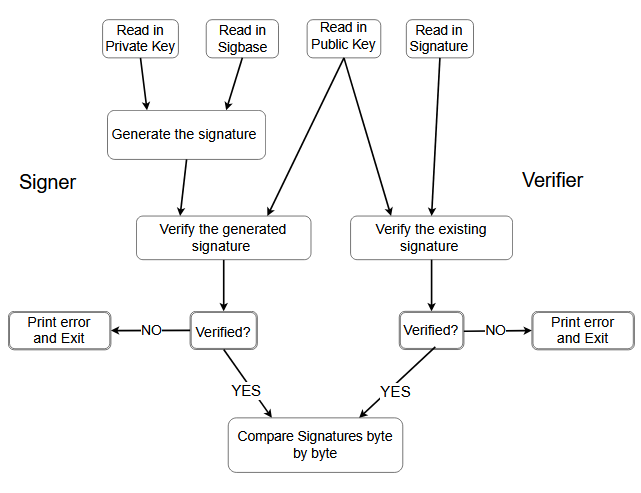
\includegraphics[height=0.5\textheight,keepaspectratio]{code/code-diagram.png}
  \caption{Flow of the DNSSEC code implementation.}
  \label{fig:code-flow}
\end{figure}
\FloatBarrier

\section{Converting Base64 Data}

To convert the Base64 signature from the file as well as the public and private keys into a format that can be used for verification, I used OpenSSL's Base64 decoding functions. 
This allows me to take the Base64-encoded signature and convert it back into its original binary format, which is necessary for the verification process. 
The code for this conversion is shown in \cref{fig:base64-code}. I enlisted Anthropic's Claude to help me with this part, and it was able 
to generate the code for me based on the OpenSSL documentation. This allowed me to focus on the actual signing and validation portions of the project,
while these utility functions were implemented with the assistance of Claude.

\begin{figure}[htbp]
  \centering
  \fbox{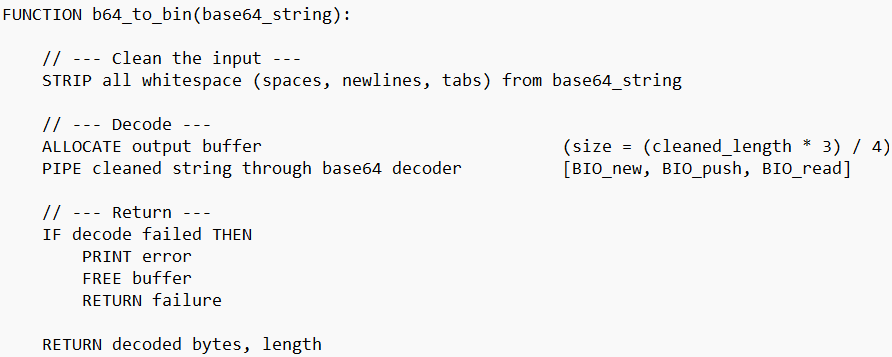
\includegraphics[width=0.8\textwidth]{code/psuedo/b64-psuedo.png}}
  \caption{Pseudocode for converting the Base64-encoded signature from the file into its original binary format using OpenSSL's Base64 decoding functions, written by Claude.}
  \label{fig:base64-code}
\end{figure}

\section{Alternative Key Encoding}

The keys that are stored on the DNSSEC servers are in a format that is not directly usable in the C code. Therefore, I had to 
convert them from the DNSSEC format to PEM format, which is a widely used format for storing cryptographic keys. I had Anthropic's Claude help 
me with this conversion and wrote code to convert the keys. This code takes both a public and private key from the .key and .private 
files from the server, and converts the keys into a .pem RSA format that can be used in the C code for signing and verifying the signatures. In \cref{fig:keys}, 
the top text is a private key straight from bind, and below is that same key in .pem format.

\begin{figure}[htbp]
  \centering
  \fbox{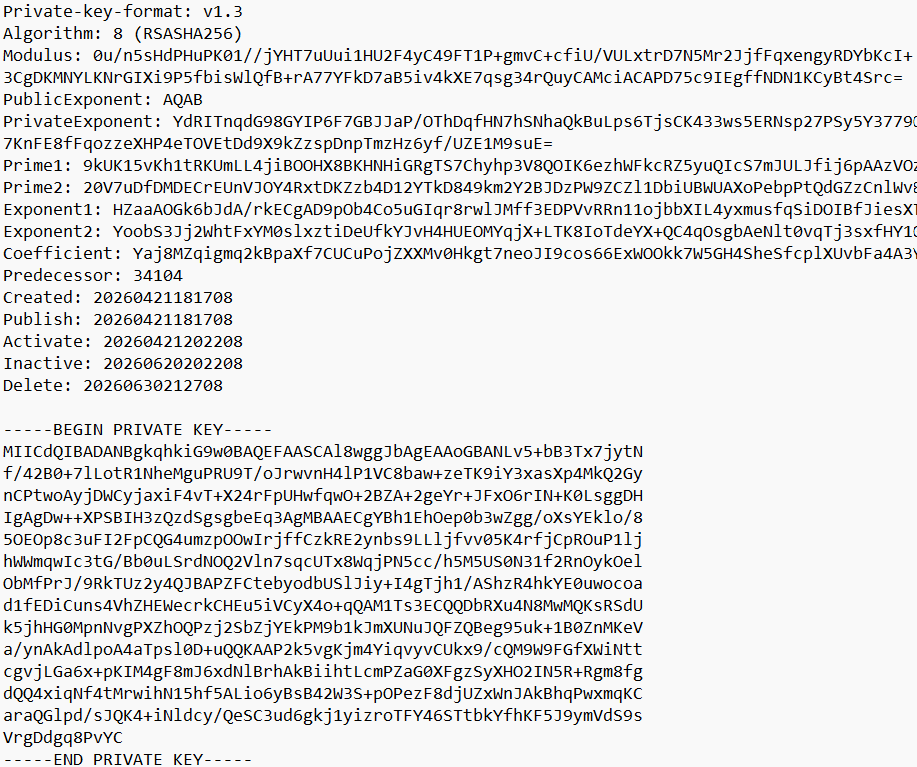
\includegraphics[width=0.7\textwidth]{code/different key formats.png}}
  \caption{A comparison between a DNSKEY private key (top) and the converted PEM format private key (bottom).}
  \label{fig:keys}
\end{figure}

\FloatBarrier

Overall, the code reads in the DNSSEC key data, determines if it is a public or private key, and then uses OpenSSL functions to convert 
the key data into the appropriate PEM format. The way the keys are stored in the .key and .private files is in a format that includes 
extra information, such as the key tag and algorithm, which is not needed for the PEM format.


\section{Hashing the Data}

To hash the data, I used OpenSSL's SHA256 algorithm. This algorithm is widely used in many cryptographic applications, and is considered to be a secure 
hashing algorithm. It produces a 256-bit hash, which is a fixed size output that is unique to the input data. This means that even a small 
change in the input data will produce a completely different hash, making it difficult for attackers to create a hash collision. The code that 
just hashes the data is shown in \cref{fig:hashing-code}.

\begin{figure}[htbp]
  \centering
  \fbox{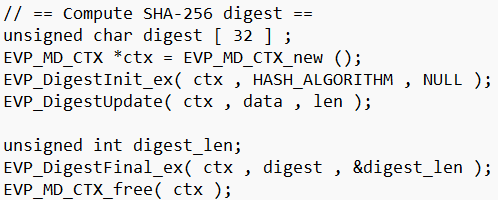
\includegraphics[width=0.8\textwidth]{code/just_hash.png}}
  \caption{Code from a helper function that hashes the data using OpenSSL's SHA256 algorithm, used for printing the hash of the data to be signed.}
  \label{fig:hashing-code}
\end{figure}

\section{Signing the Data}
\label{sec:signing}

For signing the hashed data, RSA keys were used. For signing, only the private keys were needed. The private key is used to sign the data, 
and the verification code is shown in \hyperref[sec:verify-code]{Verifying the Signature}. The code that just signs the data is shown in \cref{fig:signing-code}.\cite{evp-sign}

\begin{figure}[htbp]
  \centering
  \fbox{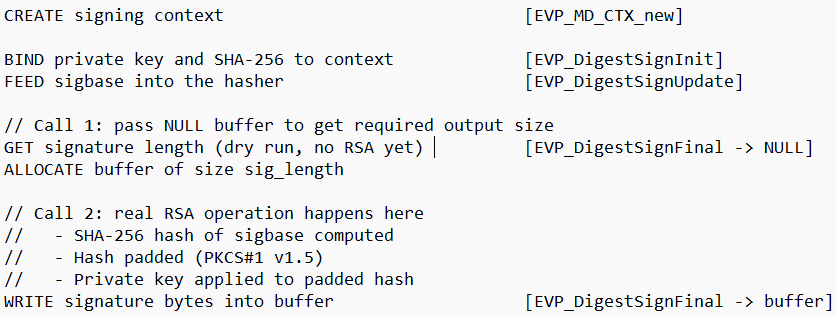
\includegraphics[width=0.9\textwidth]{code/psuedo/gen-sig-psuedo.png}}
  \caption{Pseudocode showing how the signature is created using OpenSSL's RSA signing functions. I am assuming the role of the DNS Server in this code, using the private key to sign the data.}
  \label{fig:signing-code}
\end{figure}

\section{Verifying the Signature}
\label{sec:verify-code}

The code in \cref{fig:gen-verification-code} and \cref{fig:existing-verification-code} shows how the signature is verified using OpenSSL's RSA verification 
functions, the EVP\_DigestVerify family. I am assuming the role of the DNS Client in this code, 
using the public key to verify the signatures. First, I verify the generated signature, which is the signature that I created in the previous section. 
Then, I verify the received signature, which is the signature that was read in from the file that was converted from Base64. If both of these return 
without error, both signatures are then passed to the helper function compare\_sigs.\cite{evp-verify}

\begin{figure}[htbp]
  \centering
  \fbox{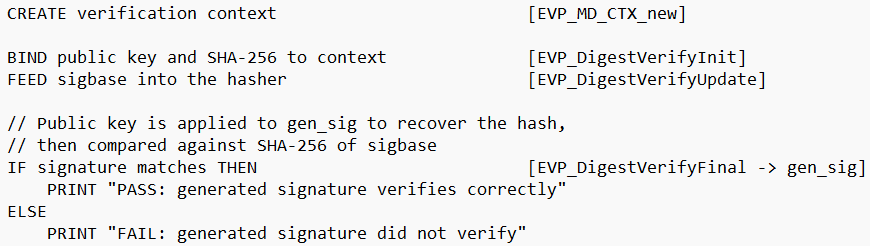
\includegraphics[width=0.9\textwidth]{code/psuedo/gen-verify-psuedo.png}}
  \caption{Pseudocode for verifying the generated signature using OpenSSL's RSA verification functions.}
  \label{fig:gen-verification-code}
\end{figure}

\begin{figure}[htbp]
  \centering
  \fbox{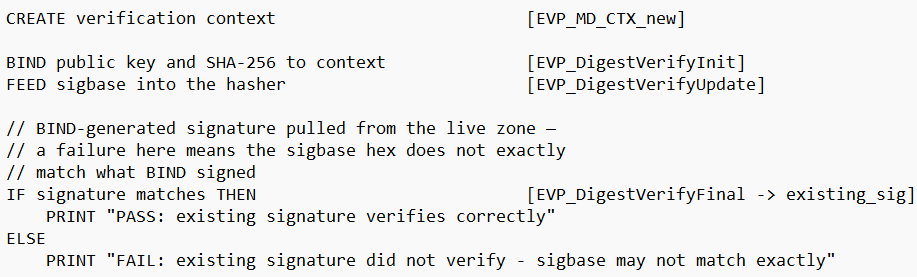
\includegraphics[width=0.9\textwidth]{code/psuedo/existing-verify-psuedo.png}}
  \caption{Pseudocode for verifying the existing signature using OpenSSL's RSA verification functions.}
  \label{fig:existing-verification-code}
\end{figure}

The final verification is a function used to compare the binaries of each signature, compare\_sigs. This is seen below in \cref{fig:comp}. 
This byte-for-byte match is also meaningful because the signing process is deterministic, meaning that the same input will always produce 
the same output. This means that if the generated signature matches the existing signature, it is a strong indication that the signing and 
verification processes are working correctly, and that the data has not been tampered with. If there is a mismatch, it could indicate an 
issue with the signing process, the verification process, or that the data has been altered in some way.

\begin{figure}[htbp]
  \centering
  \fbox{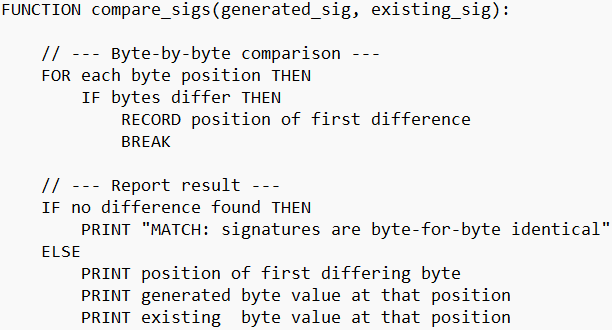
\includegraphics[width=0.8\textwidth]{code/psuedo/compare-psuedo.png}}
  \caption{{Pseudocode for the helper function that compares the generated signature and the existing signature}}
  \label{fig:comp}
\end{figure}
\FloatBarrier

\section{Tar File And Contents}

I compiled the final code into one directory, with five subdirectories containing keys, signatures, and other files. 
On the Client Virtual Machine, this code is located on the Desktop, with a copy of the tar file and the original code. 
I used the following command to tar this directory: \texttt{tar -cvf FinalCodeV1.tar \~/Desktop/Code}. To extract the files, a 
similar command is run: \texttt{tar -xvf FinalCodeV1.tar}.

\subsection{Directory Setup}

In the following sections, the set up of the different directories and what they contain are described. 
These directories are in argument order, see \cref{fig:input} above, save for the vm\_files which are used 
for key generation. A diagram of the setup is shown in \cref{fig:directory-structure} below.

\begin{figure}[htbp]
  \centering
  \fbox{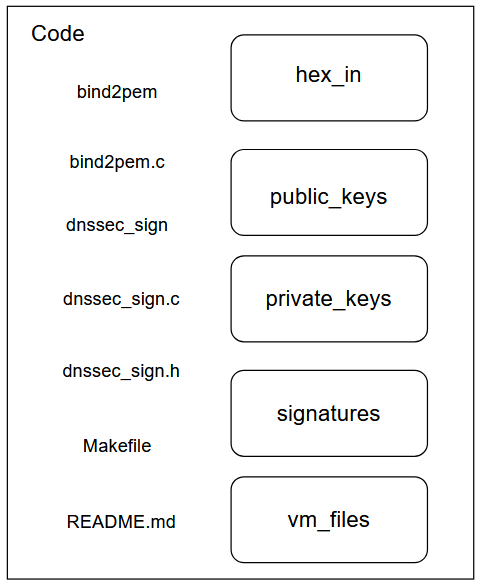
\includegraphics[width=0.6\textwidth]{code/directory-diagram.png}}
  \caption{A diagram showing the contents of the tar ball.}
  \label{fig:directory-structure}
\end{figure}

\FloatBarrier

\subsubsection{private\_keys And public\_keys}

The private\_keys and public\_keys directories contain, as the name may sound, the private and public keys for both servers in the 
environment. These keys are stored in their respective jmu-lab or lab subdirectory.


\subsubsection{hex\_in}

This directory contains the hexadecimal wire format string that the signatures are generated from. They have 
descriptive names, correlating to the record data they contain and end in a .hex extension.

\subsubsection{signatures}

The signature directory holds the base64 signatures copied straight from a dig query. The names of the files 
show what file it represents and has a .b64 extension to show that it has base64 data inside.

\subsubsection{vm\_files}

These files were pulled straight from the virtual machines, and contain the keys in their original format. These files were used to convert 
the keys into PEM format, which is used in the code for signing and verifying the signatures.

\subsection{Makefile Script}

The approach I took with the Makefile was to make a different setting for each record type that is being signed.
For each of the records, A, NS, SOA, and DNSKEY, there are separate commands for generating the signature and verifying the signature. 
There are also commands to perform cleaning, removing old executables and keys, and compiling the code. This provides a more friendly 
interface to anyone trying to use this software.

\subsubsection{Compilation}

For compiling the code, there are two commands. For the signature verification code, \texttt{make compile} creates an 
executable from the dnssec\_sign.c file. To compile the bind2pem.c file, \texttt{make compile-keys} creates the executable 
to convert the keys.

\subsubsection{Cleaning}

There are also some commands for clearing a stale executable and key files. To clear the executable, run \texttt{make clean} 
for the dnssec\_sign executable and \texttt{make clean-keys} to remove old key files.

\subsubsection{Verification}

After the keys have been generated and the code has been compiled, there are some commands to run the signature generation 
and verification. For each of the records, A, NS, SOA, and DNSKEY, there are separate commands for generating the signature and verifying the signature. 
For each of these records, a simple \texttt{make a}, \texttt{make ns}, \texttt{make soa}, and \texttt{make dnskey} will generate the 
signature and verify it against the existing signature from the server.

\section{Wire Format Construction}

\subsection{Overview}

As discussed before, the signature base consists of the RRSIG metadata, followed by the record data in wire format. The wire format is a specific 
way of encoding the DNS records into a binary format that can be used for hashing and signing. This is very important and difficult in some aspects to do, because it 
must match Bind exactly, even a small variation can lead to great error. The wire format includes the owner name, type, class, 
TTL, RDLENGTH, and RDATA for each record. This is discussed in more detail at RFC4034.\cite{rfc4034} This is also seen in the previous chapter, \cref{fig:rrsig-metadata}.

\subsection{Approach}

I captured DNSSEC traffic from the server using Wireshark, and then used the data from the capture to construct the wire format for each of the records. I copied out the whole answer section as a hex dump, then extracted data that way.
This was a difficult process, as the wire format is very specific and any small mistake can lead to a completely different hash and signature. Wireshark allowed 
me to extract the raw bytes of fields and put them together. Wireshark also compresses the names of the records using pointer bytes, like 0xc0 0x0c, which have to be 
expanded to the full wire format before being placed into the signature base. This is seen in \cref{fig:wireshark-name} below, where the compressed name is shown, as well as the expanded name in the data section. 
As an example of name expansion: for the name ns.jmu.lab., the compressed format was 0x02 (length) 0x6e73 (data) 0xc00c (pointer) in Wireshark, 
but the expanded format is 0x02 0x6e73 (ns)0x03 0x6a6d75 (jmu) 0x03 0x6c6162 (lab) 0x00 (end), which is the full wire format for the name.\cite{rfc4034}


\begin{figure}[htbp]
  \centering
  \fbox{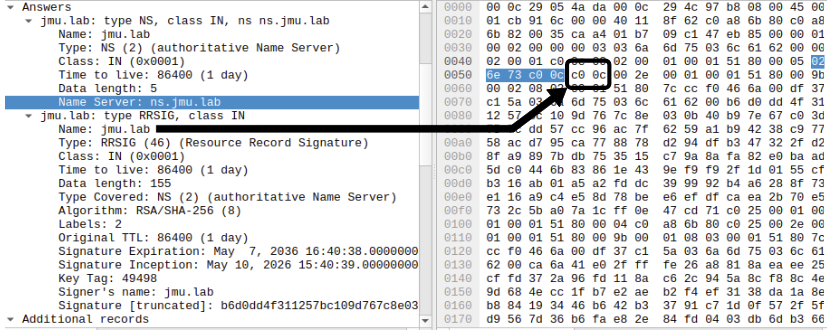
\includegraphics[width=\textwidth]{code/wireshark/wireshark-name.png}}
  \caption{A screenshot of Wireshark showing a compressed name, as well as other data in order. You can see in the blue highlighted area is the name server's name, with the uncompressed ns and the compressed pointer for the rest of the name.}
  \label{fig:wireshark-name}
\end{figure}
\FloatBarrier

\subsection{Commonalities And Exceptions}

There are some commonalities between the different record types, specifically in the RRSIG headers. In general, there are 18 bytes minimum, from the type covered 
(2 bytes), algorithm (1 byte), labels (1 byte), original TTL (4 bytes), signature expiration (4 bytes), signature inception (4 bytes), key tag (2 bytes), and 
signer's name (variable length). In the case of \cref{fig:rrsig-diagram} below, the signer name is jmu.lab., meaning the full header length is 27 total bytes. 
The 0x00 at the end of the names indicates the end of the name and that it is a FQDN.

\begin{figure}[htbp]
  \centering
  \fbox{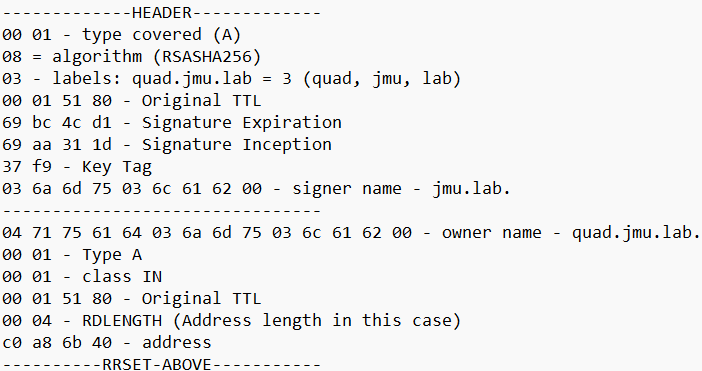
\includegraphics[width=0.8\textwidth]{code/rrsig.png}}
  \caption{A diagram showing the header and data for an Address record signature.}
  \label{fig:rrsig-diagram}
\end{figure}
\FloatBarrier

Some challenges that I faced when constructing the wire format for the different records were getting the timestamp conversions correct. The compressed names were a 
bit tricky at first, but it wasn't so bad when I figured out what was going on. The timestamps are shown in YYYYMMDDhhmmss format, and converting them to the 
correct hex format was a bit difficult, but I was able to convert it by running a command like \texttt{date -d "2026-05-12 12:00:00" -u +\%s} to get the Unix timestamp, 
then converting that to hex and making sure it was in the correct byte order with a command like \texttt{printf "\%08x" <timestamp>}. The -u flag is passed to get the 
timestamp in UTC, which is important for the signature to be valid.\cite{rfc4034}


\section{Generating and Validating an Address Resource Record Signature}

The Address Resource Record Signature is the most basic signature. This signature consists of the RRSIG meta data, describing what record is 
being signed and the logistics of the signature, like TTL and an expiration date among others. Appended to the header, is the owner name (e.g. computer.lab.), type, class, 
TTL, RDLENGTH, specifying the length of the RDATA payload, in this case 4 for IPv4, then four bytes for the IP. For computer.lab, it would look like this: 
192.168.107.2 becomes c0 a8 6b 02. As seen before, in \cref{fig:rrsig-metadata}, this shows an Address records data. Below, in \cref{fig:a-verification}, is the 
output from my code, showing the matching signatures.

\begin{figure}[htbp]
  \centering
  \fbox{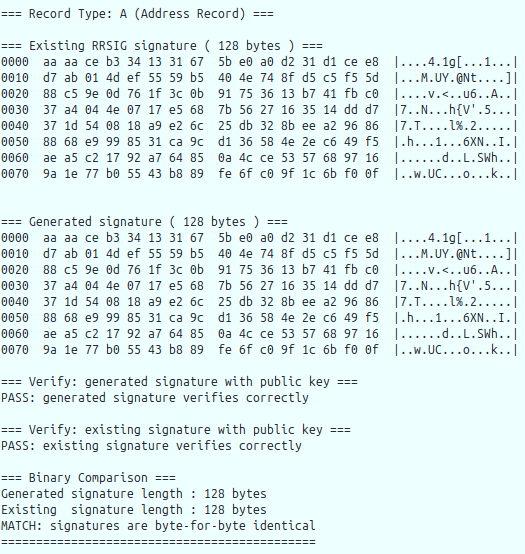
\includegraphics[width=0.7\textwidth]{code/new-a-output.png}}
  \caption{Output from validating an A RRSIG record.}
  \label{fig:a-verification}
\end{figure}

\FloatBarrier

\section{Generating and Validating a Name Server Resource Record Signature}

The Name Server Resource Record was a bit more tricky than the Address Record Signature. After the signature header, once again the owner name follows,
(e.g. jmu.lab.), then the type (0x0002), class IN (0x0001), the TTL, the RDLENGTH and the RDATA. For the jmu.lab server, the length of the RDATA would 
be 12 bytes, or 0x000c in hex, and the RDATA is ns.jmu.lab., which becomes 0x02 0x6e73 (ns) 0x03 0x6a6d75 (jmu) 0x03 0x6c6162 (lab) 0x00 in hex.\cite{rfc4034}

\begin{figure}[htbp]
  \centering
  \fbox{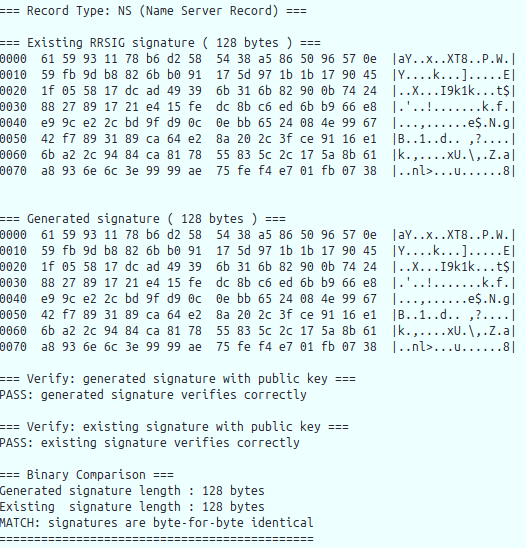
\includegraphics[width=0.7\textwidth]{code/new-ns-output.png}}
  \caption{Output from validating an NS RRSIG record.}
  \label{fig:ns-verification}
\end{figure}

\FloatBarrier

\section{Generating and Validating a DNSKEY Resource Record Signature}

The DNSKEY Resource Record Signature is the biggest and one of the more difficult records to sign. This signature requires the KSK to be used, 
as the DNSKEYs are being signed, which means that these keys are to be passed to the program. The KSK is double the size of the ZSKs, 
and this leads to a doubly large signature. The output of this record is seen below in \cref{fig:dnskey-verification}. The signature length 
expands to 256 bytes long from the previous 128 byte zone records.

Following the meta data of the RRSIG, the DNSKEY record has some unique data appended to it. It starts the same as the other records, with 
the owner name, type (0x0030 in this instance), class, and TTL of the record. Then the RDLENGTH is passed, and it is a combination of the 
two byte flags (0x0101 for KSK [257] and 0x0100 for ZSK [256]), single byte protocol, and single byte algorithm, followed by the raw key 
bytes of the public key, decoded from base64, which is 260 bytes long for the KSK and 132 bytes long for the ZSK, for a total of 264 bytes 
for the KSK and 136 bytes for the ZSK. This is seen below in \cref{fig:dnskey-rdata}. 


\begin{figure}[htbp]
  \centering
  \fbox{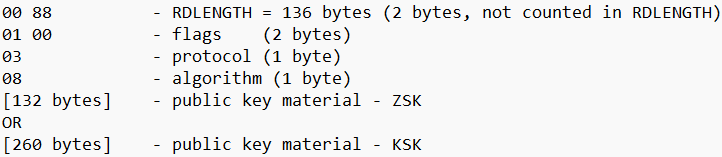
\includegraphics[width=0.9\textwidth]{code/dnskey-diagram.png}}
  \caption{A diagram showing the RDATA of the DNSKEY records.}
  \label{fig:dnskey-rdata}
\end{figure}

The reason for the larger than usual size of the keys is because the public exponent is encoded and 
sent in a specific format, which adds 4 extra bytes. It is the first four bytes of the public key material, the exponent length, 0x03, and 
the public exponent, 0x010001. This is seen in \cref{fig:wireshark-key}. Both the public KSK 
and ZSK are passed, so they must be canonically ordered. Using Wireshark, the KSK was shown first in the message in the wire response, but the 
sigbase requires canonical ordering. Since the ZSK flag value 0x0100 sorts lexicographically before the KSK flag value 0x0101, 
placing the ZSK first in the signature base per RFC 4034.\cite{rfc4034}

\begin{figure}[htbp]
  \centering
  \fbox{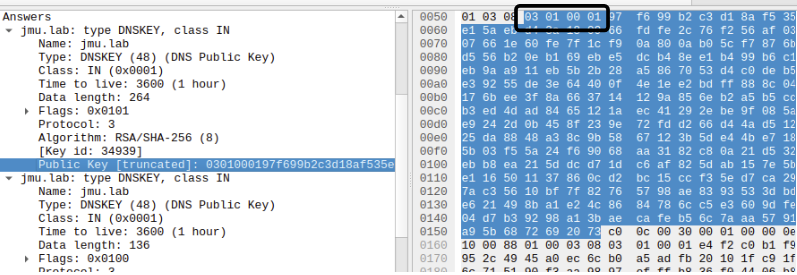
\includegraphics[width=\textwidth]{code/wireshark/dnskey-wireshark.png}}
  \caption{Wireshark traffic showing the first four bytes of the public key material, followed by the rest of the key.}
  \label{fig:wireshark-key}
\end{figure}

\begin{figure}[htbp]
  \centering
  \fbox{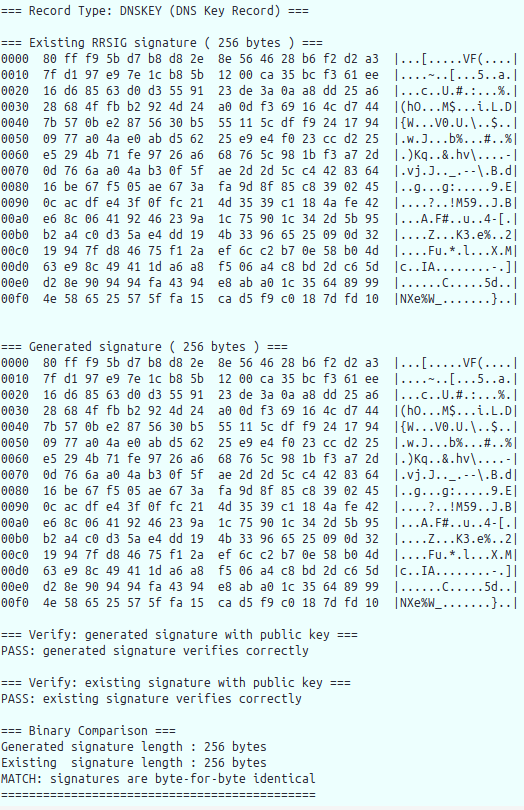
\includegraphics[width=0.6\textwidth]{code/new-dnskey-output.png}}
  \caption{Output from validating a DNSKEY RRSIG record.}
  \label{fig:dnskey-verification}
\end{figure}

\FloatBarrier

\section{Generating and Validating a Start of Authority Resource Record Signature}

The Start of Authority Resource Record signature was one of the most difficult to construct. It started off the same as the others, 
with the owner name, type (0x0006), class, and TTL. The RDLENGTH is variable, and depends on the length of both the MNAME and RNAME. 
The MNAME is the primary nameserver, and the RNAME is the responsible mailbox, seen below in \cref{fig:soa-ex}. Following those, there are 
five fixed length fields, which can be seen too.

\begin{figure}[htbp]
  \centering
  \fbox{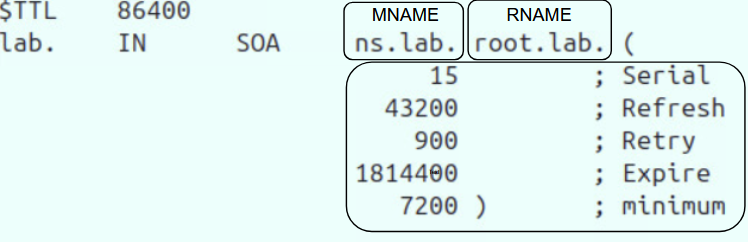
\includegraphics[width=0.7\textwidth]{code/soa-example.png}}
  \caption{An example of a SOA record for my lab zone, showing the RNAME and MNAME, as well as the other fields.}
  \label{fig:soa-ex}
\end{figure}

\FloatBarrier

All of these records are four bytes long, starting with 
the serial number, refresh, retry, expire, and minimum fields. A problem I ran into when constructing the data for this record 
was having the serial number wrong, as it gets incremented every time a zone reload occurs. The serial number must be captured at the same moment as the signature.
This is a field in the Wireshark output and dig, which makes it easier to keep track of, but needs to be kept up to date. The hardest part for me was getting the correct MNAME and RNAME 
values and having them in fully expanded wire format, then adding them to the RDLENGTH. Getting the RDLENGTH wrong by even one 
byte results in a completely wrong value. The output from my code when generating and validating an SOA signature is seen in 
\cref{fig:soa-verification} below.\cite{rfc4034}

\begin{figure}[htbp]
  \centering
  \fbox{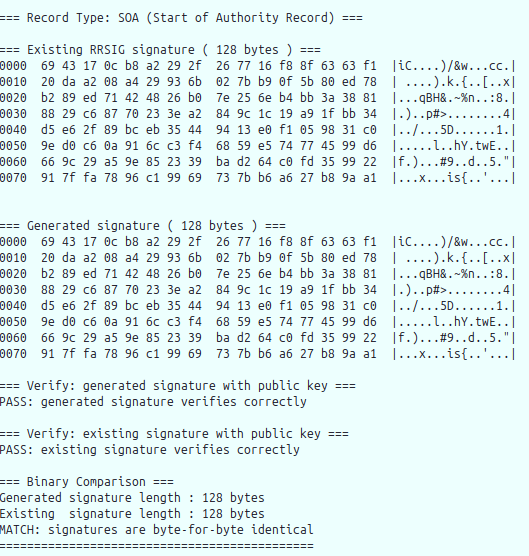
\includegraphics[width=0.7\textwidth]{code/new-soa-output.png}}
  \caption{Output from validating a SOA RRSIG record.}
  \label{fig:soa-verification}
\end{figure}

\FloatBarrier

% \section{Conclusion}
% % Make more chapter oriented?
% The four records shown above 

% this project was a great learning experience for me. It was a lot of fun to work on, and I learned a lot about 
% DNSSEC and how it works. I enjoyed exploring more into DNS and DNSSEC, as well as investigating deeper into the vulnerabilities 
% and attacks on DNS, as well as manually validating the signatures. Coding the signatures really helped me understand the 
% process of how the signatures are generated and validated, as well as the importance of the wire format and how it is constructed 
% and the security that is provided by them. 